\documentclass{article}
\usepackage{amsmath,amssymb,bm}
\usepackage{algorithm,algpseudocode}
\usepackage{graphicx}

\setlength{\paperwidth}{210mm}
\setlength{\paperheight}{297mm}
\setlength{\voffset}{0mm}
\setlength{\textwidth}{\paperwidth}
\addtolength{\textwidth}{-30mm}
\setlength{\textheight}{\paperheight}
\addtolength{\textheight}{-60mm}
\setlength{\topmargin}{-1in}
\addtolength{\topmargin}{20mm}
\setlength{\headheight}{0mm}
\setlength{\headsep}{0mm}
\setlength{\footskip}{20mm}
\setlength{\oddsidemargin}{-1in}
\addtolength{\oddsidemargin}{15mm}
\setlength{\columnsep}{7mm}

\title{\large {\bf Memo: Back-propagation}}
\author{Tomomichi Sugihara}

\everymath{\displaystyle}

\begin{document}
\maketitle

\begin{figure}[h]
\centering
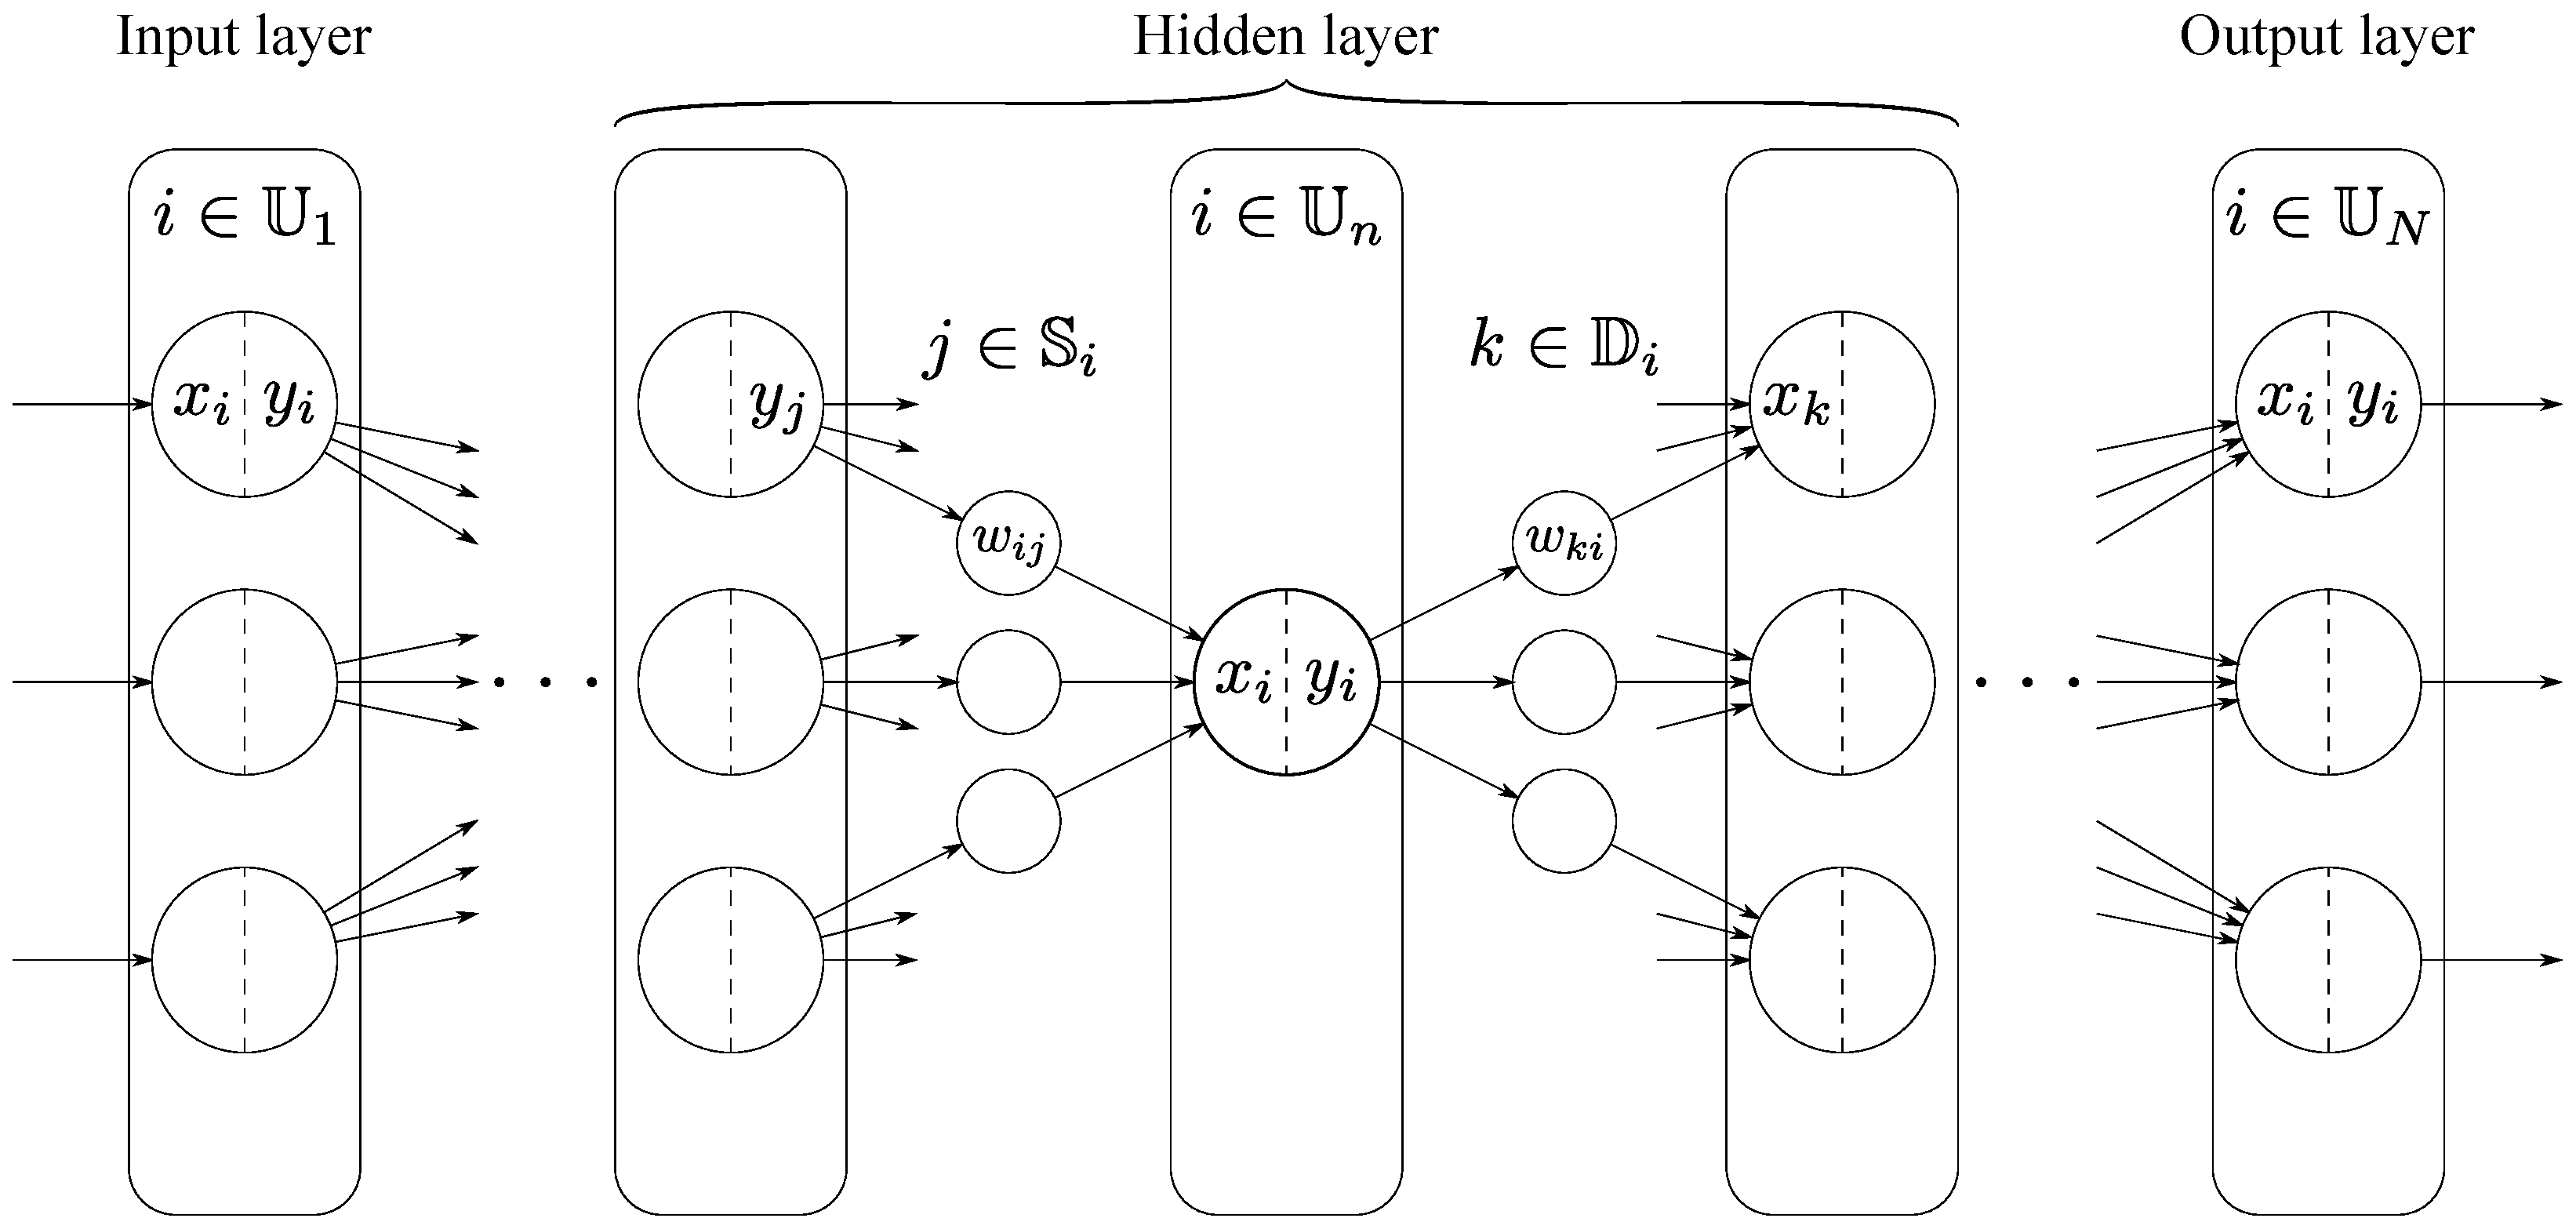
\includegraphics[width=.7\textwidth]{multilayerednetwork.eps}
\caption{A non-recurrent multi-layered neural network}
\label{fig:multilayerednetwork}
\end{figure}

Let us consider a non-recurrent $N$-layered neural network
illustrated in Fig. \ref{fig:multilayerednetwork}.
The transmission of information in it is represented by the following equations:
\begin{align}
x_{i}&=\begin{cases}
\mbox{given} & \mbox{(if $i\in\mathbb{U}_{1}$)} \\
\sum_{j\in\mathbb{S}_{i}}w_{ij}y_{j}+b_{i} & \mbox{(otherwise)}
\end{cases}
\\
y_{i}&=\begin{cases}
x_{i} & \mbox{(if $i\in\mathbb{U}_{1}$)} \\
f_{i}(x_{i}), & \mbox{(otherwise)}
\end{cases}
\end{align}
where
$x_{i}$ is the input to the $i$th neural unit,
$\mathbb{U}_{n}$ for $n=1, \cdots, N$ is the set of indices of units in the $n$th layer,
$\mathbb{S}_{i}$ is the set of indices of upstream neural units connected to the $i$th unit,
$y_{i}$ is the output of the $i$th unit,
$w_{ij}$ is the weight on $y_{j}$ that is input to the $i$th unit,
$b_{i}$ is the bias of the $i$th unit,
and $f_{i}(\cdot)$ is the activation function associated with the $i$th unit.
By propagating the output of each unit from the input layer to the output layer
based on the above equations,
the network transforms the input $\bm{x}=\{x_{i}|\forall i\in\mathbb{U}_{1}\}$
to the output $\bm{y}=\{y_{i}|\forall i\in\mathbb{U}_{N}\}$.
Namely, it represents a multi-input-multi-output algebraic mapping
$\mathcal{N}_{\{w_{ij}\},\{b_{i}\}}:\bm{x}\mapsto\bm{y}$ or $\bm{y}=\bm{F}(\bm{x})$.

Provided an input $\bm{x}^{*}$ paired with the desired output $\bm{y}^{*}$,
the loss function of the network $E(\bm{x}^{*},\bm{y}^{*};\mathcal{N}_{\{w_{ij}\},\{b_{i}\}})$ is defined.
A typical choice of the function is the sum of squared errors as
\begin{align}
E(\bm{x}^{*},\bm{y}^{*};\mathcal{N}_{\{w_{ij}\},\{b_{i}\}})\overset{\mathrm{def}}{=}
\frac{1}{2}\left\|\bm{F}(\bm{x}^{*})-\bm{y}^{*}\right\|^{2}.
\end{align}
The back-propagation is one of the representative methods
to train the network, \textit{i.e.}, all the weights $\{w_{ij}\}$ and the biases $\{b_{i}\}$
so as to minimize the above loss function
based on the following update rule:
\begin{align}
w_{ij}&\leftarrow w_{ij}-\eta\varDelta w_{ij}
\\
b_{i}&\leftarrow b_{i}-\eta\varDelta b_{i},
\end{align}
where
$\eta$ is the learning rate.
$\varDelta w_{ij}$ and $\varDelta b_{i}$ are decided
to align the steepest descent direction as
\begin{align}
\varDelta w_{ij}&=\frac{\partial E_{\mathbb{L}}}{\partial w_{ij}} \\
\varDelta b_{i}&=\frac{\partial E_{\mathbb{L}}}{\partial b_{i}},
\end{align}
where
$E_{\mathbb{L}}$ is the following loss function of a mini-batch
\begin{align}
E_{\mathbb{L}}=\sum_{l\in\mathbb{L}}E(\bm{x}^{*(l)},\bm{y}^{*(l)};\mathcal{N}_{\{w_{ij}\},\{b_{i}\}}),
\end{align}
$\mathbb{L}$ is the set of identifiers of runs included in the mini-batch,
$\bm{x}^{*(l)}$ is the input in the $l$th run to the network,
and $\bm{y}^{*(l)}$ is the corresponding desired output of the network.
Obviously,
\begin{align}
\frac{\partial E_{\mathbb{L}}}{\partial w_{ij}}
&=\sum_{l\in\mathbb{L}}\frac{\partial E}{\partial w_{ij}}(\bm{x}^{*(l)},\bm{y}^{*(l)};\mathcal{N}_{\{w_{ij}\},\{b_{i}\}})
\\
\frac{\partial E_{\mathbb{L}}}{\partial b_{i}}
&=\sum_{l\in\mathbb{L}}\frac{\partial E}{\partial b_{i}}(\bm{x}^{*(l)},\bm{y}^{*(l)};\mathcal{N}_{\{w_{ij}\},\{b_{i}\}}),
\end{align}
and hence,
the goal here is to find
$\frac{\partial E}{\partial w_{ij}}$
and $\frac{\partial E}{\partial b_{i}}$.

\bigskip

$w_{ij}$ and $b_{i}$ only affect $x_{i}$ directly, and thus,
\begin{align}
\frac{\partial E}{\partial w_{ij}}
&=
\frac{\partial E}{\partial x_{i}}
\frac{\partial x_{i}}{\partial w_{ij}}
=
p_{i}y_{j}
\\
\frac{\partial E}{\partial b_{i}}
&=
\frac{\partial E}{\partial x_{i}}
\frac{\partial x_{i}}{\partial b_{i}}
=
p_{i},
\end{align}
where
\begin{align}
p_{i}\overset{\mathrm{def}}{=}
\frac{\partial E}{\partial x_{i}}.
\end{align}
$x_{i}$ affects $y_{i}$,
and $y_{i}$ affects $\{x_{k}|\forall k\in\mathbb{D}_{i}\}$,
where $\mathbb{D}_{i}$ is the set of indices of downstream units connected to the $i$th unit,
if it belongs to a hidden layer.
Hence,
\begin{align}
p_{i}
=\frac{\partial E}{\partial y_{i}}\frac{\partial y_{i}}{\partial x_{i}}
=\begin{cases}
\frac{\partial E}{\partial y_{i}}f_{i}^{\prime}(x_{i})
& \mbox{(if $i\in\mathbb{U}_{N}$)}
\\
\left(\sum_{k\in\mathbb{D}_{i}}\frac{\partial E}{\partial x_{k}}\frac{\partial x_{k}}{\partial y_{i}}\right)
\frac{\partial y_{i}}{\partial x_{i}}
=\left(\sum_{k\in\mathbb{D}_{i}}p_{k}w_{ki}\right)f_{i}^{\prime}(x_{i}).
& \mbox{(otherwise)}
\end{cases}
\end{align}
In the typical case of the sum of squared errors,
\begin{align}
\frac{\partial E}{\partial y_{i}}
=y_{i}-y_{i}^{*}
\qquad\mbox{for}\quad
\forall i\in\mathbb{U}_{N}.
\end{align}
$f_{i}^{\prime}(x_{i})$ depends on the definition of $f_{i}(x_{i})$.
If it is the sigmoid function,
\begin{align}
f_{i}(x_{i})=\frac{1}{1+e^{-x_{i}}}
\qquad\Rightarrow\qquad
f_{i}^{\prime}(x_{i})=\frac{e^{-x_{i}}}{\left(1+e^{-x_{i}}\right)^{2}}=y_{i}\left(1-y_{i}\right).
\end{align}
Or, if it is ReLU,
\begin{align}
f_{i}(x_{i})=\max\left\{x_{i},0\right\}
\qquad\Rightarrow\qquad
f_{i}^{\prime}(x_{i})=\begin{cases}
1 & \mbox{(if $x_{i}\geq 0$)}
\\
0 & \mbox{(otherwise)}
\end{cases}.
\end{align}
Note that ReLU is not differentiable at $x_{i}=0$ in the strict sense,
although it is usually ignored.

A pseudocode of an algorithm for a neural network $\mathcal{N}_{\{w_{ij}\},\{b_{i}\}}$
to train from data set $\left\{\left.(\bm{x}^{*(l)},\bm{y}^{*(l)})\right|\forall l\in\mathbb{L}\right\}$
and the loss function $E(\bm{x}^{*},\bm{y}^{*};\mathcal{N}_{\{w_{ij}\},\{b_{i}\}})$
based on the above back-propagation is as follows.
\begin{algorithm}
\caption{\textsc{TrainNN}$(\mathcal{N}_{\{w_{ij}\},\{b_{i}\}},\left\{\left.(\bm{x}^{*(l)},\bm{y}^{*(l)})\right|\forall l\in\mathbb{L}\right\},\eta)$}
\begin{algorithmic}[1]
\Require $\mathcal{N}_{\{w_{ij}\},\{b_{i}\}} \cdots$ initialized
\Ensure $\mathcal{N}_{\{w_{ij}\},\{b_{i}\}} \cdots$ updated
\State \textsc{InitGrad}$(\mathcal{N}_{\{w_{ij}\},\{b_{i}\}})$ \Comment{Initialize gradients of weights and biases}
\For{$l\in\mathbb{L}$} \Comment{Evaluate each run in a mini-batch}
  \State \textsc{BackPropagate}$(\mathcal{N}_{\{w_{ij}\},\{b_{i}\}},(\bm{x}^{*(l)},\bm{y}^{*(l)}))$
\EndFor
\State \textsc{UpdateNN}$(\mathcal{N}_{\{w_{ij}\},\{b_{i}\}},\eta)$ \Comment{Update weights and biases of neural network}
\end{algorithmic}
\end{algorithm}

\begin{algorithm}
\caption{\textsc{InitGrad}$(\mathcal{N}_{\{w_{ij}\},\{b_{i}\}})$}
\begin{algorithmic}[1]
\For{$i\in\mathbb{U}_{2}\cup\cdots\cup\mathbb{U}_{N}$}
  \For{$j\in\mathbb{S}_{i}$}
    \State $\varDelta w_{ij}\leftarrow 0$
  \EndFor
  \State $\varDelta b_{i}\leftarrow 0$
\EndFor
\end{algorithmic}
\end{algorithm}

\begin{algorithm}
\caption{\textsc{BackPropagate}$(\mathcal{N}_{\{w_{ij}\},\{b_{i}\}},(\bm{x}^{*(l)},\bm{y}^{*(l)}))$}
\begin{algorithmic}[1]
\Ensure $\{\varDelta w_{ij}\},\{\varDelta b_{i}\}$
\State \textsc{Propagate}$(\mathcal{N}_{\{w_{ij}\},\{b_{i}\}},\bm{x}^{*(l)})$
\State \textsc{InitParam}$(\mathcal{N}_{\{w_{ij}\},\{b_{i}\}})$
\For{$i\in\mathbb{U}_{N}$} \Comment{for output layer}
  \State $p_{i}\leftarrow {\partial E}/{\partial y_{i}}(\bm{x}^{*(l)},\bm{y}^{*(l)};\mathcal{N}_{\{w_{ij}\},\{b_{i}\}})$ (dependent on the definition of $E$)
\EndFor
\For{$n=N$ downto $2$} \Comment{Backpropagation}
  \For{$i\in\mathbb{U}_{n}$}
    \State $p_{i}\leftarrow p_{i}v_{i}$
    \State $\varDelta d_{i}\leftarrow\varDelta d_{i}+p_{i}$
    \For{$j\in\mathbb{S}_{i}$}
      \State $p_{j}\leftarrow p_{j}+p_{i}w_{ij}$
      \State $\varDelta w_{ij}\leftarrow\varDelta w_{ij}+p_{i}y_{j}$
    \EndFor
  \EndFor
\EndFor
\end{algorithmic}
\end{algorithm}

\begin{algorithm}
\caption{\textsc{InitParam}$(\mathcal{N}_{\{w_{ij}\},\{b_{i}\}})$}
\begin{algorithmic}[1]
\For{$i\in\mathbb{U}_{1}\cup\cdots\cup\mathbb{U}_{N}$}
  \State $p_{i}\leftarrow 0$
  \State $v_{i}\leftarrow f^{\prime}(x_{i})$
\EndFor
\end{algorithmic}
\end{algorithm}

\begin{algorithm}
\caption{\textsc{UpdateNN}$(\mathcal{N}_{\{w_{ij}\},\{b_{i}\}},\eta)$}
\begin{algorithmic}[1]
\Require $\{\varDelta w_{ij}\},\{\varDelta b_{i}\} \cdots$ computed
\Ensure $\{w_{ij}\},\{b_{i}\} \cdots$ updated
\For{$i\in\mathbb{U}_{2}\cup\cdots\cup\mathbb{U}_{N}$}
  \State $d_{i}\leftarrow d_{i}-\eta\varDelta d_{i}$
  \For{$j\in\mathbb{S}_{i}$}
    \State $w_{ij}\leftarrow w_{ij}-\eta\varDelta w_{ij}$
  \EndFor
\EndFor
\end{algorithmic}
\end{algorithm}


\end{document}
